\section{Backtracking}

\subsection{Descripcion del problema}

	El problema consiste en formar el grupo más grande de agentes comfiables para esto se cuenta con una tabla que representa las encuestas hechas a los agentes. La primera columna de dicha tabla representa el agente encuestado mientras que la segunda columna representa lo que dicho agente informó. Además, cada agente puede elegir informar algo como no, y si lo hace puede hacer tantas declaraciones como desee. Luego la tabla puede ser vacía como tener muchas entradas (notar que la tabla no puede ser infinita). Una vez hechas todas las encuestas se procede a decir cuál es el grupo más grande de agentes confiables. No todo conjunto de agentes es válido por lo que hay ciertas propiedades que tiene que cumplir. La primera es que si un agente dentro del conjunto confía en otro agente, ese agente también debe estar en el grupo, la segunda es que si un agente dentro del conjunto desconfia de otro agente, este no puede ester en el conjunto. Algunos ejemplos serían:
	
\begin{table}[H]
\begin{tabular}{c c}
Agentes & Encuestas  \\ [0.5ex]
\hline
1 & 2 \\
2 & 3 \\
3 & -1 \\
0 & 0 \\ [1ex]
\hline
res: 2 \\
\end{tabular}
\end{table}

\begin{table}[h]
\begin{tabular}{c c}
\centering
Agentes & Encuestas \\ [0.5ex]
\hline
1 & 5 \\
2 & 3 \\
3 & 4 \\
5 & -1 \\ [1ex]
\hline
res: 3 \\
\end{tabular}
\end{table}

\subsection{Solución Propuesta}

	La idea para resolver este problema es considerar todos los posibles casos. Para esto vimos que cada agente puede estar como no en el conjunto, o sea, se va a analizar ambos conjuntos resultantes, uno donde el agente esté en el conjunto y otro donde no esté. A la hora de agregar un agente, llamémoslo i, al conjunto primero vemos que se pueda, esto significa que va a seguir siendo un conjunto válido, para esto vamos a ver un par de cosas. La primera es que nadie en el conjunto desconfíe de i, luego veremos que i no desconfíe de nadie que está en el conjunto, también se verifica que la encuesta del agente tenga sentido lógico, o sea, que no desconfíe de si mismo y, como puede hacer más de una declaración, que no desconfie y confie de un agente. Además para la rama en la cuál no se agrega al agente vereficamos que tenga sentido que no este en el conjunto, esto es que nadie, que este en el conjunto, confie en él. Una vez hecho esto, y  para los otros posibles conjuntos válidos, se elegirá el conjunto con mayor cantidad de agentes. 
	
\subsection{Resolución}
	La técnica de backtracking consiste en pensar conceptualmente en un árbol que contega todas las posibles soluciones. Por esto la solución que propone mi algoritmo es la siguiente:
	
\begin{itemize}
\setlength\itemsep{-0.2em}
\item Partir de la raíz (ningún agente elegido).
\item Comenzar por el primer agente ver si puede ser agregado al conjunto (las consideraciones descriptas en el punto anterior) y considerar que no forme parte del mismo, luego recorrer recursivamente cada una de esas 2 posibilidades para el elemento siguiente (2 ramas).
\item A partir del segundo elemento, recorrer recursivamente cada una de las 2 ramas sólo si ésta es válida, en otras palabras, si puede ser agregado el agente al conjunto. Además si el agente tiene que estar en el conjunto (porque alguien en el conjunto confía en él) la rama que corresponde a no agregar al agente no se recorre ya que no sería una instancia válida del problema.
\item Al llegar a una hoja que esté en el último nivel (cuando la altura del árbol es igual a la cantidad de agentes) se chequea que el conjunto resultante sea válido esto lo hacemos por que a la hora de agregar un agente al conjunto no estamos viendo que si este confia en alguien que no esta en el conjunto se pueda agregar a ese agente en el futuro. Luego si la cantidad de agentes dentro del conjunto resultante es mayor a la que ya tenés, entonces ésta será la mejor solución. Si no, entonces me quedo con la solución que tenía antes.
\end{itemize}
	
\subsection{Pseudocódigo}

\begin{algorithm}[H]
\caption{Backtracking}\label{Ej1}

\begin{algorithmic}[H]
\Procedure{Backtracking}{vector(pair(agente, agente)) encuestas, agentes, ConjAgentes}
\If{Si no me quedan agentes para evaluar}
\If{longitud(ConjAgentes) > solucion}
\State solucion $=$ longitud(ConjAgentes)
\EndIf
\EndIf
\If{PuedoAgregarAgente}
\State Paso Recursivo rama agregueAlAgente
\EndIf
\If{NadieConfiaEnElAgente}
\State Paso Recursivo rama NoAgregoAlAgente
\EndIf
\EndProcedure
\end{algorithmic}
\end{algorithm}

	A la hora de recorrer ambas ramas, se verifica que no genere instancias inválidas. Lo que hacen las guardas de los ifs es comprobar esa validez.
\subsection{Demostración de correctitud}

	La técnica descripta anteriormente parte de pensar al problema como un árbol con todas las posibles soluciones. Cada nodo del árbol representa como se va ir modificando nuestro conjunto incluyendo o no a un determinado agente. A pesar de que nuestro algoritmo se basa en esta idea falta decir porque es correcto respecto a nuestro problema ya que como dijimos antes no recorre todos los casos. La razón es que recorre las ramas que son válidas según las condiciones del problema y no considera las inválidas. Una vez que tenemos el conjunto de soluciones posibles se queda con la mejor de ellas, en este paso (cuando ya se recorrió todo el árbol) se podrían considerar las soluciones descartadas pero serían descartas de nuevo, ya que no cumplen con lo pedido, lo que hacemos es descartalas antes de llegar al final del árbol para ahorrarnos recorrer dichas ramas. Entonces al final generamos todas las posibles soluciones y nos quedamos con la mejor.

\subsection{Complejidad teórica}
	
	Como dijimos antes la idea conceptual del problema es pensarlo como un árbol de soluciones. Como este árbol contempla todas las posibles soluciones es un árbol completo, ya que por cada nodo tenemos 2 opciones, que forme parte del conjunto o que no forme (no hace falta considerar cuando alguna rama no es recorridas ya que estamos considerando complejidad en peor caso, por lo que  consideramos el árbol completo). Entonces terminamos teniendo un árbol con $2^{i}$ hojas, donde "i" es la cantidad de agentes. Además para pasar de un nivel del árbol a otro, pagamos O($a^{2}*i$) esto se debe a que vemos las encuestas del agente evaluado y las encuestas de los agentes que ya pertenecen al conjunto y chequeamos que cumplan lo descripto anteriormente. Esto lo hacemos cuando queremos ver si un agente es confiable, para la rama que no es confiable pagamos O($a$) para ver si efectivamente el agente evaluado puede no pertenecer al conjunto, luego nos queda la suma de las complejidades O(($a^{2}*i$) + ($a^{2}*i$)) donde nos quedamos con la más grande. Luego en el último nivel hacemos un chequeo para ver si efectivamente el conjunto es válido, esto se debe a que a la hora de agregar un agente al conjunto no estamos considerando que si éste confía en un agente y ese agente no se encuentra en el conjunto lo pueda agregar en el futuro. Para hacer esto tenemos que recorrer una vez mas el conjunto y ver que siga siendo un conjunto válido. Esto nos toma O($i^{2}a$) pasos. Luego, una vez recorrido todo el árbol, terminamos teniendo una complejidad de O($2^{i}*((i*a^{2})+(i^{2}*a))$).
	
\subsection{Experimentación} 
	
	Para analizar la performancia del algoritmo decidimos considerar diferentes entradas. Cada entrada consiste en fijar la cantidad de agentes (yendo desde 1 agente hasta 20) y tomar 100 repeticiones para la cantidad fijada. Cada repetición toma una cantidad de encuestas igual a la cantidad de agentes lo que nos queda es una relación 1 a 1, y las encuestas son elegidas de forma aleatoria. Entonces, por ejemplo, tenemos 100 repeticiones para un agente con un encuesta random, luego 100 repeticiones para 2 agentes y asi sucesivamente, una vez tomadas todas las muestras se corre el algoritmo y se toma el tiempo que tarda. Una vez que se tienen los tiempos se toma un promedio de ellos. Las entradas que consideramos fueron, una donde todas las encuestas son positivas, una donde todas las encuestas son negativas y por último una donde se elige aleatoriamente si la encuesta es positiva o negativa.       
	
\begin{figure}[h]
\begin{subfigure}{0.5\textwidth}
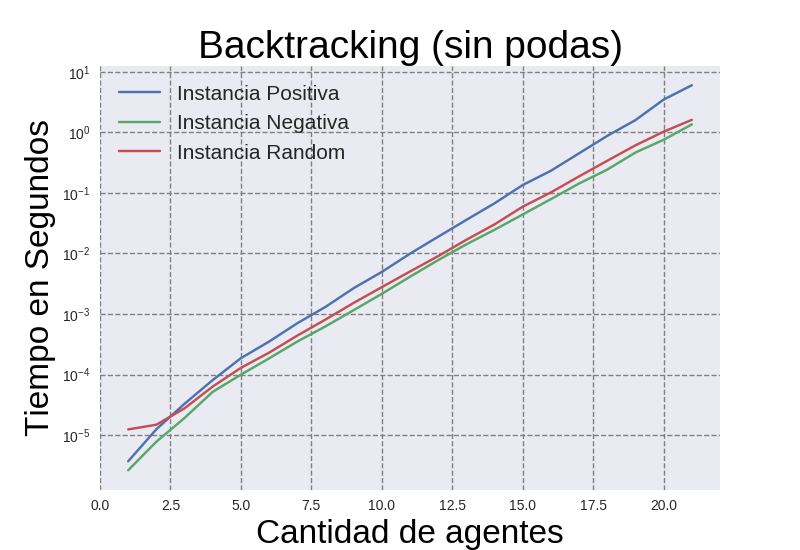
\includegraphics[scale=0.45]{BacktrackingLog.png}
\end{subfigure}
\begin{subfigure}{0.5\textwidth}
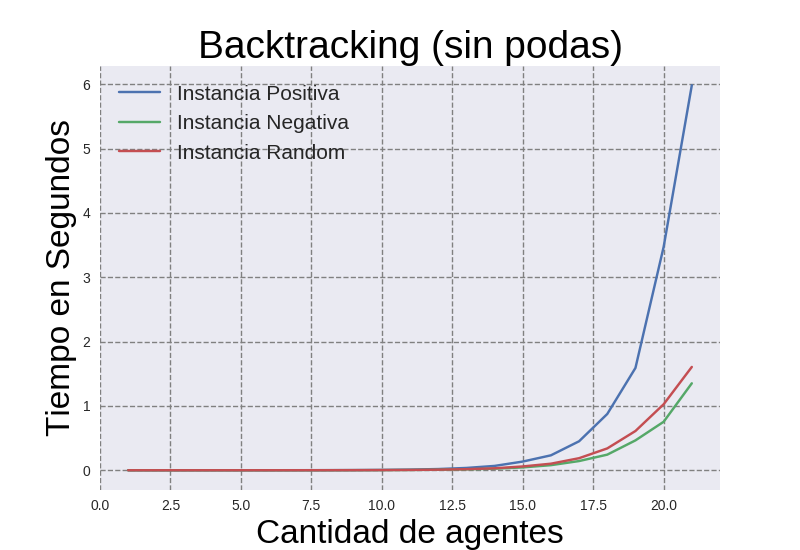
\includegraphics[scale=0.45]{Backtracking.png}
\end{subfigure}
\end{figure}

	En los gráficos podemos ver que la peor instancia es la postiva, esto se debe a que recorremos todas las ramas donde agregamos un agente al conjunto ya que todas las encuestas son positivas. Lo que no estaríamos recorriendo en esta instancia serían los casos donde queremos ver si podemos no agregar un agente al conjunto, ya que es posible que otro agente en el conjunto confie en él. Pero en general estaríamos recorriendo casi todo el árbol. Para las otras instacias no se ve un diferencia muy grande.
	
	Para el segundo experimento lo que hicimos fue fijar el número de agentes a 18 e ir aumentando el número de encuestas hasta llegar a una proporción de 2 a 1. Con esto queríamos ver si a medida que aumentamos las encuestas, estas influyen en el tiempo del algoritmo. Las encuestas fueron elegidas aleatoriamente tanto el voto en si como si es positiva o negativa. El método de medición fue el mismo que utilizamos en la experimentación anterior.
	 
	\begin{figure}[h]
	\begin{subfigure}{0.5\textwidth}
	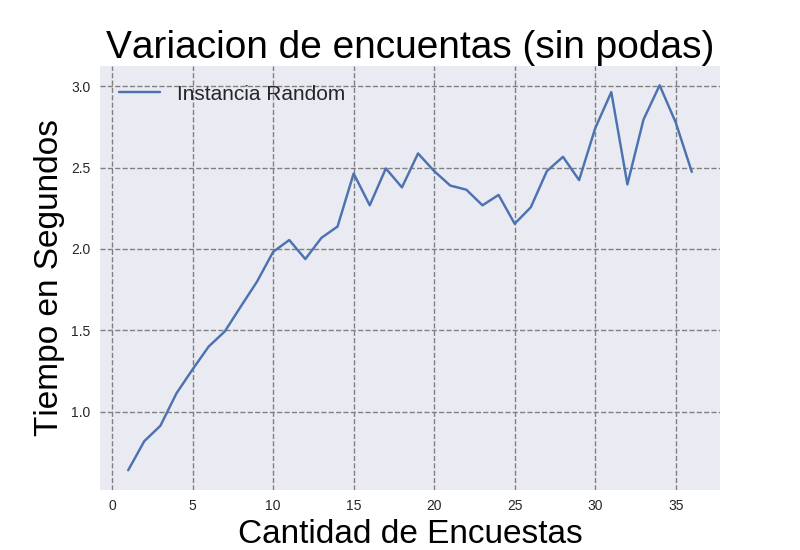
\includegraphics[scale=0.45]{VariacionesSinPodas.png}	
	\end{subfigure}
	\end{figure} 
	
	Lo que sacamos del gráfico es el aumento del tiempo en relación al aumento de las encuestas.
	\\	
	
	\begin{figure}[h]
	\begin{subfigure}{0.5\textwidth}
	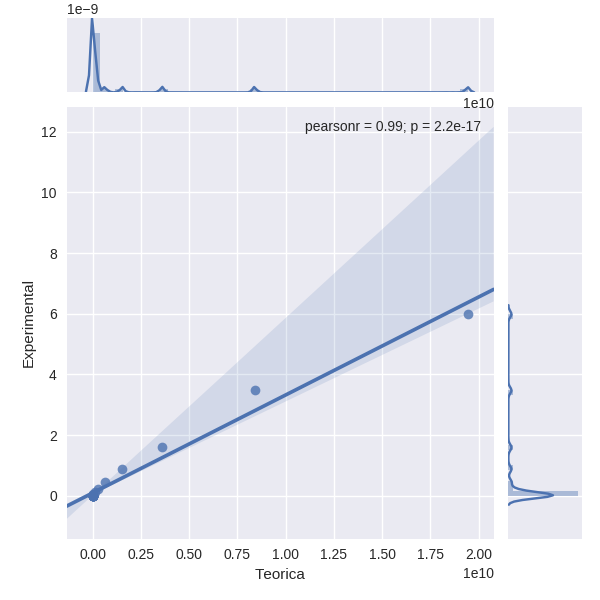
\includegraphics[scale=0.45]{Pearson.png}	
	\end{subfigure}
	\end{figure}  
	
	Por último quisimos comparar nuestra función teórica de complejidad con los resultados empíricos de nuestro algoritmo. Para esto utilizamos los resultados de la instancia positiva que, como vimos, es el peor caso para nuestro algoritmo y es lo que más se asemeja a la complejidad en peor caso. Para realizar la comparación utilizamos el coeficiente de Pearson. Este nos dice si dos variables tiene una relación o no. 
	
	
	 
	
	En el gráfico podemos ver una relación directa casi perfecta, esto nos dice que los resultados de nuestro algoritmo y de la fución teórica se comportan de manera similiar, esto quiere decir que cuando uno aumenta el otro también lo hace. 
	 
	



